\documentclass[t]{beamer}

%\documentclass[handout, t]{beamer}
\setbeamertemplate{navigation symbols}{}
\usepackage{pstricks}
\usepackage{mathtools}
\usepackage{amsfonts}
\usepackage{mathrsfs}
\usepackage{amsmath}
\usepackage{physics}
\setbeamertemplate{navigation symbols}{}
\usepackage{bm}
\usepackage[UTF8]{ctex}
\usetheme{AnnArbor}
\usefonttheme{serif}
\useinnertheme{rounded}
\usecolortheme{beaver}
\setbeamertemplate{blocks}[rounded][shadow=true]

\newcommand{\dif}{{\;\rm d}}
\usepackage{graphicx}
\usepackage{pgf}
\usepackage{tikz}
\usetikzlibrary{arrows, decorations.pathmorphing, backgrounds, positioning, fit, petri, automata}
\tikzset{>=stealth}

\usepackage{setspace}
\setmainfont{Times New Roman}
\setCJKmainfont{Microsoft YaHei}


\hypersetup{pdfpagemode=FullScreen}
\renewcommand{\Pr}{\mathbb{P}}
\usepackage{blkarray}


\setbeamercolor{block title}{bg=red!10!white}
\setbeamercolor{block body}{bg=gray!10!white}

\usepackage{multicol}
\newcommand{\E}{\mathbb{E}}
\newcommand{\EP}{\mathbb{E}^{\mathbb{P}}}
\newcommand{\EQ}{\mathbb{E}^{\mathbb{Q}}}
\newcommand{\Var}{{\rm Var}}
\newcommand{\Cov}{{\rm Cov}}


\begin{document}
\fontsize{11}{18}\selectfont


\CTEXindent



  \title{第六章~~布朗运动}
\author{随机过程及其在金融中的应用}
\date{中国人民大学出版社}
  \begin{frame}
    \maketitle
  \end{frame}

  \begin{frame}{引言}
    离散时间马氏链的状态和时间均是离散的;而连续时间马氏链则是状态离散、时间连续的。实际上,还有一类满足马氏性,并且时间和状态均连续的随机过程,称为马氏过程(Markov process),其中最具有代表性的就是在金融工程、高能物理等研究领域中被广泛使用的布朗运动。

    \begin{center}
      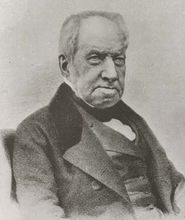
\includegraphics[height=.35\textheight]{fig/brown.jpg} 
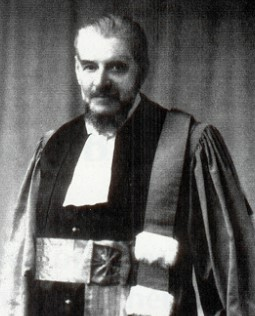
\includegraphics[height=.35\textheight]{fig/bachelier.jpg}
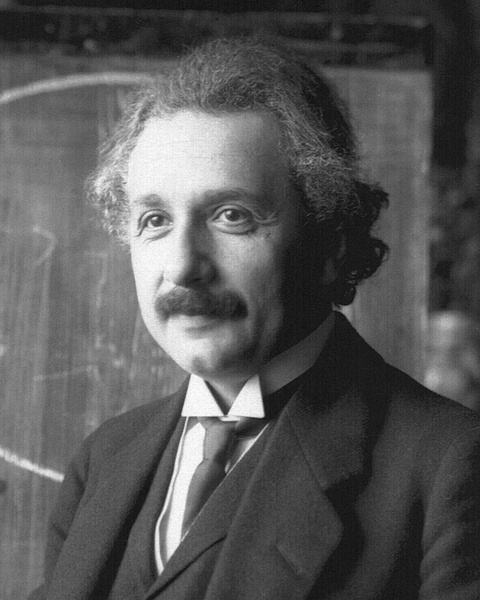
\includegraphics[height=.35\textheight]{fig/einstein.jpg}
\includegraphics[height=.35\textheight]{fig/wiener.jpeg}
    \end{center}
  \end{frame}

\begin{frame}{布朗运动简史}
  布朗运动(Brownian motion)是由英国生物学家罗伯特·布朗(Robert Brown,1773---1858)于1828年首
先观察到的花粉颗粒浮于液体内不规则运动的物理现象。
1900年,法国数学家路易斯·巴舍利耶(Louis Bachelier,1870---1946)在他的博士论文中正式将布朗运动
引入证券市场,用来描述股价的变动。阿尔伯特·爱因斯坦(Albert Einstein,1879---1955)于1905年在研究狭义相对论的过程中,独立地对布朗运动进行了数学刻画。之后,诺伯特·维纳(Norbert Wiener,1894---1964)在1923 年研究了布
朗运动的数学理论,并对其严格定义,因此布朗运动也被称为维纳过程(Wiener process)。
\end{frame}

\begin{frame}{布朗运动简史(cont.)}
  美国经济学家保罗· 萨缪尔森(Paul Samuelson,1915---2009)在曼德尔布罗特(B. Mandelbrot,1924---2010)和奥斯本(M. F. Osborne,1888---1966)的启发下,于1960年代对巴舍利耶的研究成果进行了重新发掘,将
布朗运动再度引入
金融经济学模型,并尝试
研究金融市场中的权证定价问题。
至此,布朗运动在金融经济学及金融工程学中建立了重要地位。
\begin{center}
  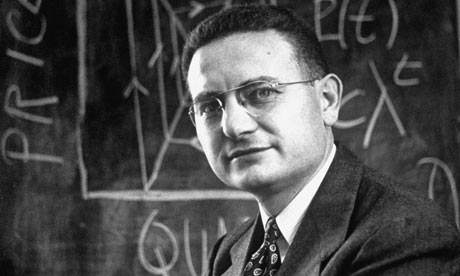
\includegraphics[scale=.5]{fig/Samuelson.jpg}
\end{center}
\end{frame}

\begin{frame}{本章内容}\small
\begin{spacing}{1.2}
  \begin{multicols}{2}
    \tableofcontents
  \end{multicols} 
\end{spacing} 
\end{frame}


\section{随机游走}

\subsection{随机游走的含义}


\begin{frame}{随机游走的含义}
  假设一个粒子每隔$\Delta t$时间做一次向上或向下的运动,其中向上运动的概率为$p$,移动的距离为$1$个单位;向下运动的概率为$q=1-p$,移动的距离也为$1$个单位。将粒子向上运动的方向记为正值,则相应地粒子向下运动的位移即为$-1$个单位。将每次粒子的位移记作随机变量$Z_i$,其中$i$表示移动的次数。相应地,粒子的上下运动称作随机游走(random walk)。因此有:
  \begin{equation*}
  \Pr(Z_i=1)=p,\qquad \Pr(Z_i=-1)=q=1-p
  \end{equation*}
  
  假设随机变量$Z_i$是独立同分布的,当$t=n\Delta t$时,将$t$时间段内粒子的位移记作$X(t)$,则有:
  \begin{equation*}
  X(t)=Z_1+Z_2+\cdots +Z_n
  \end{equation*}
\end{frame}


\begin{frame}{随机游走的含义(cont.)}
  因此:\[\begin{split}
    \E(Z_i)&=1 \cdot \Pr(Z_i=1)+(-1)\cdot \Pr(Z_i=-1)=p-q\\
    \E(Z_i^2)&=1^2 \cdot \Pr(Z_i=1)+(-1)^2\cdot \Pr(Z_i=-1)=1\\
    \Var(Z_i)&=\E(Z_i^2)-[\E(Z_i)]^2=4pq
    \end{split}
    \]
    由于期望具有线性性质,因此:
\begin{equation*}
\E[X(t)]=\E(Z_1)+\E(Z_2)+\cdots +\E(Z_n)=n(p-q)
\end{equation*}
另外,基于随机变量$Z_i$是独立同分布的前提假设可得:
\begin{equation*}
\Var[X(t)]=\Var(Z_1)+\Var(Z_2)+\cdots +\Var(Z_n)=4npq
\end{equation*}
\end{frame}


\begin{frame}{随机游走示意图}
  \centering
  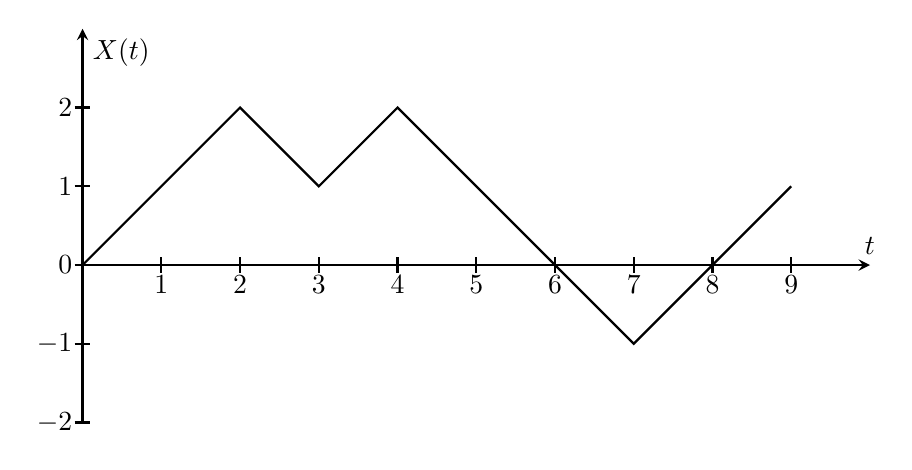
\begin{tikzpicture}[>=stealth, thick, scale=1]
    \draw[->] (0,-2) --(0,3);
    \draw[->] (0,0)--(10,0);
    
    \node at (10,0)[above]{$t$};
    \node at (0,2.7)[right]{$X(t)$};
    
    
    \foreach \x in {-2,-1,0, 1,2}
    {\draw(-.1, \x)--(.1,\x);
    \node  at (0,\x) [left] {$\x$}; }
    
    \foreach \y in {1,2,3,4,5,6,7,8,9}
    {\draw(\y, .1)--(\y, -.1);
    \node  at (\y,0) [below] {$\y$}; }
    
    \draw (0,0)--(1,1)--(2,2)--(3,1)--(4,2)--(5,1)--(6,0)--(7,-1)--(8,0)--(9,1);
    
    \end{tikzpicture}
\end{frame}

\subsection{对称随机游走}
\begin{frame}{对称随机游走}
  若随机游走的粒子上下运动的概率均为50\%,即$p=q=0.5$,可以得到粒子位移$X(t)$的均值和方差分别为:
  \begin{equation*}
  \begin{split}
  \E[X(t)]&=n(p-q) = 0\\
  \Var[X(t)]&=4npq=n
  \end{split}
  \end{equation*}
  对应的每次粒子位移$Z_i$的均值和方差分别为:
  \begin{equation*}
  \E(Z_i)=0,\qquad \Var(Z_i)=1
  \end{equation*}
  此时的随机游走称作对称随机游走(symmetric random walk)。
其中,$n=t/\Delta t$,也就是$t$时间段粒子位移的次数。

\begin{block}{}\centering
  位移的期望为零,方差则与位移次数$n$有关。
\end{block}
\end{frame}

\begin{frame}{对称随机游走的二次变差}
  截至$t$时刻的对称随机游走的二次变差(quadratic variation)定义如下:
  \begin{equation*}
  \langle X,X\rangle(t) =\sum^{n}_{i=1}(X_i-X_{i-1})^2
  \end{equation*}
  由于增量$Z_i=X_i-X_{i-1}=\pm 1$,因此:
  \begin{equation*}
  \langle X,X\rangle(t) =n
  \end{equation*}
  由此不难看出,对称随机游走的二次变差在数值上等于其方差,即:
  \begin{equation*}
  \Var[X(t)]=n=\langle X,X\rangle(t)
  \end{equation*}
\end{frame}


\begin{frame}{对称随机游走的二次变差与方差}
  \begin{equation*}
    \Var[X(t)]=n=\langle X,X\rangle(t)
    \end{equation*}

    二次变差$\langle X,X\rangle(t)=n$与随机游走中上下运动的概率无关;而方差$\Var[X(t)]=n$成立的前提是对称随机游走,即$p=q=0.5$。
    
    正因如此,二次变差$\langle X,X\rangle(t)$是沿着随机游走的单条路径计算得到,而方差$\Var[X(t)]$则是对所有的路径,以其概率权重求平均得到。
\end{frame}

\subsection{按比例缩小型对称随机游走}
\begin{frame}{按比例缩小型对称随机游走}
  在原先的对称随机游走的基础上,引入按比例缩小型对称随机游走(scaled symmetric random walk),将原先的$t$时间段粒子位移的次数$n$划分成更小的时间段,假设这里将每个时间段$\Delta t=t/n$划分成距离相等的$m$段,则每个时间段就由$\Delta t$变为$\Delta t/m$,相应地粒子位移的次数由$n$次变为$mn$次。在此基础上,将原先每次位移的长度由$Z_i$变为$W^{(m)}(s)$,从而可得:
  \begin{equation*}
  W^{(m)}(s)=\frac{1}{\sqrt{m}}Z_{ms},\qquad s\in[0,t]
  \end{equation*}
\end{frame}


\begin{frame}{按比例缩小型对称随机游走的示意图}
  \centering
  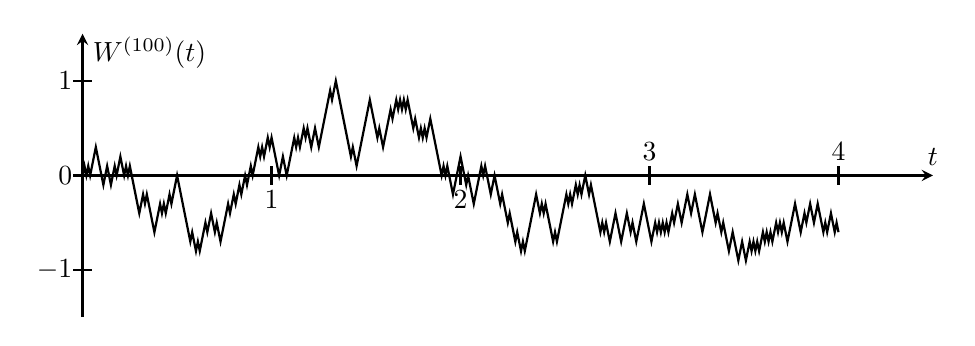
\begin{tikzpicture}[>=stealth, thick, scale=1.2]
  \draw[->] (0,-1.5) --(0,1.5);
  \draw[->] (0,0)--(9,0);
  
  \node at (9,0)[above]{$t$};
  \node at (0,1.3)[right]{$W^{(100)}(t)$};
  
  
  \foreach \x in {-1,0,1}
  {\draw(-.1, \x)--(.1,\x);
  \node  at (0,\x) [left] {$\x$}; }
  
  \foreach \y in {2,4,6,8}
  {\draw(\y, .1)--(\y, -.1);
  }
  
  \node  at (2,-.25)  {1}; 
  \node  at (4,-.25)  {2}; 
  \node  at (6,.25) {3}; 
  \node  at (8,.25) {4}; 
  
  \draw (0, 0)--(0.02, 0.1)--(0.04, 0)--(0.06, 0.1)--(0.08, 0)--(0.1, 0.1)--(0.12, 0.2)--(0.14, 0.3)--(0.16, 0.2)--(0.18, 0.1)--(0.2, 0)--(0.22, -0.1)--(0.24, 0)--(0.26, 0.1)--(0.28, 0)--(0.3, -0.1)--(0.32, 0)--(0.34, 0.1)--(0.36, 0)--(0.38, 0.1)--(0.4, 0.2)--(0.42, 0.1)--(0.44, 0)--(0.46, 0.1)--(0.48, 0)--(0.5, 0.1)--(0.52, 0)--(0.54, -0.1)--(0.56, -0.2)--(0.58, -0.3)--(0.6, -0.4)--(0.62, -0.3)--(0.64, -0.2)--(0.66, -0.3)--(0.68, -0.2)--(0.7, -0.3)--(0.72, -0.4)--(0.74, -0.5)--(0.76, -0.6)--(0.78, -0.5)--(0.8, -0.4)--(0.82, -0.3)--(0.84, -0.4)--(0.86, -0.3)--(0.88, -0.4)--(0.9, -0.3)--(0.92, -0.2)--(0.94, -0.3)--(0.96, -0.2)--(0.98, -0.1)--(1, 0)--(1.02, -0.1)--(1.04, -0.2)--(1.06, -0.3)--(1.08, -0.4)--(1.1, -0.5)--(1.12, -0.6)--(1.14, -0.7)--(1.16, -0.6)--(1.18, -0.7)--(1.2, -0.8)--(1.22, -0.7)--(1.24, -0.8)--(1.26, -0.7)--(1.28, -0.6)--(1.3, -0.5)--(1.32, -0.6)--(1.34, -0.5)--(1.36, -0.4)--(1.38, -0.5)--(1.4, -0.6)--(1.42, -0.5)--(1.44, -0.6)--(1.46, -0.7)--(1.48, -0.6)--(1.5, -0.5)--(1.52, -0.4)--(1.54, -0.3)--(1.56, -0.4)--(1.58, -0.3)--(1.6, -0.2)--(1.62, -0.3)--(1.64, -0.2)--(1.66, -0.1)--(1.68, -0.2)--(1.7, -0.1)--(1.72, 0)--(1.74, -0.1)--(1.76, 0)--(1.78, 0.1)--(1.8, 0)--(1.82, 0.1)--(1.84, 0.2)--(1.86, 0.3)--(1.88, 0.2)--(1.9, 0.3)--(1.92, 0.2)--(1.94, 0.3)--(1.96, 0.4)--(1.98, 0.3)--(2, 0.4)--(2.02, 0.3)--(2.04, 0.2)--(2.06, 0.1)--(2.08, 0)--(2.1, 0.1)--(2.12, 0.2)--(2.14, 0.1)--(2.16, 0)--(2.18, 0.1)--(2.2, 0.2)--(2.22, 0.3)--(2.24, 0.4)--(2.26, 0.3)--(2.28, 0.4)--(2.3, 0.3)--(2.32, 0.4)--(2.34, 0.5)--(2.36, 0.4)--(2.38, 0.5)--(2.4, 0.4)--(2.42, 0.3)--(2.44, 0.4)--(2.46, 0.5)--(2.48, 0.4)--(2.5, 0.3)--(2.52, 0.4)--(2.54, 0.5)--(2.56, 0.6)--(2.58, 0.7)--(2.6, 0.8)--(2.62, 0.9)--(2.64, 0.8)--(2.66, 0.9)--(2.68, 1)--(2.7, 0.9)--(2.72, 0.8)--(2.74, 0.7)--(2.76, 0.6)--(2.78, 0.5)--(2.8, 0.4)--(2.82, 0.3)--(2.84, 0.2)--(2.86, 0.3)--(2.88, 0.2)--(2.9, 0.1)--(2.92, 0.2)--(2.94, 0.3)--(2.96, 0.4)--(2.98, 0.5)--(3, 0.6)--(3.02, 0.7)--(3.04, 0.8)--(3.06, 0.7)--(3.08, 0.6)--(3.1, 0.5)--(3.12, 0.4)--(3.14, 0.5)--(3.16, 0.4)--(3.18, 0.3)--(3.2, 0.4)--(3.22, 0.5)--(3.24, 0.6)--(3.26, 0.7)--(3.28, 0.6)--(3.3, 0.7)--(3.32, 0.8)--(3.34, 0.7)--(3.36, 0.8)--(3.38, 0.7)--(3.4, 0.8)--(3.42, 0.7)--(3.44, 0.8)--(3.46, 0.7)--(3.48, 0.6)--(3.5, 0.5)--(3.52, 0.6)--(3.54, 0.5)--(3.56, 0.4)--(3.58, 0.5)--(3.6, 0.4)--(3.62, 0.5)--(3.64, 0.4)--(3.66, 0.5)--(3.68, 0.6)--(3.7, 0.5)--(3.72, 0.4)--(3.74, 0.3)--(3.76, 0.2)--(3.78, 0.1)--(3.8, 0)--(3.82, 0.1)--(3.84, 0)--(3.86, 0.1)--(3.88, 0)--(3.9, -0.1)--(3.92, -0.2)--(3.94, -0.1)--(3.96, 0)--(3.98, 0.1)--(4, 0.2)--(4.02, 0.1)--(4.04, 0)--(4.06, -0.1)--(4.08, 0)--(4.1, -0.1)--(4.12, -0.2)--(4.14, -0.3)--(4.16, -0.2)--(4.18, -0.1)--(4.2, 0)--(4.22, 0.1)--(4.24, 0)--(4.26, 0.1)--(4.28, 0)--(4.3, -0.1)--(4.32, -0.2)--(4.34, -0.1)--(4.36, 0)--(4.38, -0.1)--(4.4, -0.2)--(4.42, -0.3)--(4.44, -0.2)--(4.46, -0.3)--(4.48, -0.4)--(4.5, -0.5)--(4.52, -0.4)--(4.54, -0.5)--(4.56, -0.6)--(4.58, -0.7)--(4.6, -0.6)--(4.62, -0.7)--(4.64, -0.8)--(4.66, -0.7)--(4.68, -0.8)--(4.7, -0.7)--(4.72, -0.6)--(4.74, -0.5)--(4.76, -0.4)--(4.78, -0.3)--(4.8, -0.2)--(4.82, -0.3)--(4.84, -0.4)--(4.86, -0.3)--(4.88, -0.4)--(4.9, -0.3)--(4.92, -0.4)--(4.94, -0.5)--(4.96, -0.6)--(4.98, -0.7)--(5, -0.6)--(5.02, -0.7)--(5.04, -0.6)--(5.06, -0.5)--(5.08, -0.4)--(5.1, -0.3)--(5.12, -0.2)--(5.14, -0.3)--(5.16, -0.2)--(5.18, -0.3)--(5.2, -0.2)--(5.22, -0.1)--(5.24, -0.2)--(5.26, -0.1)--(5.28, -0.2)--(5.3, -0.1)--(5.32, 0)--(5.34, -0.1)--(5.36, -0.2)--(5.38, -0.1)--(5.4, -0.2)--(5.42, -0.3)--(5.44, -0.4)--(5.46, -0.5)--(5.48, -0.6)--(5.5, -0.5)--(5.52, -0.6)--(5.54, -0.5)--(5.56, -0.6)--(5.58, -0.7)--(5.6, -0.6)--(5.62, -0.5)--(5.64, -0.4)--(5.66, -0.5)--(5.68, -0.6)--(5.7, -0.7)--(5.72, -0.6)--(5.74, -0.5)--(5.76, -0.4)--(5.78, -0.5)--(5.8, -0.6)--(5.82, -0.5)--(5.84, -0.6)--(5.86, -0.7)--(5.88, -0.6)--(5.9, -0.5)--(5.92, -0.4)--(5.94, -0.3)--(5.96, -0.4)--(5.98, -0.5)--(6, -0.6)--(6.02, -0.7)--(6.04, -0.6)--(6.06, -0.5)--(6.08, -0.6)--(6.1, -0.5)--(6.12, -0.6)--(6.14, -0.5)--(6.16, -0.6)--(6.18, -0.5)--(6.2, -0.6)--(6.22, -0.5)--(6.24, -0.4)--(6.26, -0.5)--(6.28, -0.4)--(6.3, -0.3)--(6.32, -0.4)--(6.34, -0.5)--(6.36, -0.4)--(6.38, -0.3)--(6.4, -0.2)--(6.42, -0.3)--(6.44, -0.4)--(6.46, -0.3)--(6.48, -0.2)--(6.5, -0.3)--(6.52, -0.4)--(6.54, -0.5)--(6.56, -0.6)--(6.58, -0.5)--(6.6, -0.4)--(6.62, -0.3)--(6.64, -0.2)--(6.66, -0.3)--(6.68, -0.4)--(6.7, -0.5)--(6.72, -0.4)--(6.74, -0.5)--(6.76, -0.6)--(6.78, -0.5)--(6.8, -0.6)--(6.82, -0.7)--(6.84, -0.8)--(6.86, -0.7)--(6.88, -0.6)--(6.9, -0.7)--(6.92, -0.8)--(6.94, -0.9)--(6.96, -0.8)--(6.98, -0.7)--(7, -0.8)--(7.02, -0.9)--(7.04, -0.8)--(7.06, -0.7)--(7.08, -0.8)--(7.1, -0.7)--(7.12, -0.8)--(7.14, -0.7)--(7.16, -0.8)--(7.18, -0.7)--(7.2, -0.6)--(7.22, -0.7)--(7.24, -0.6)--(7.26, -0.7)--(7.28, -0.6)--(7.3, -0.7)--(7.32, -0.6)--(7.34, -0.5)--(7.36, -0.6)--(7.38, -0.5)--(7.4, -0.6)--(7.42, -0.5)--(7.44, -0.6)--(7.46, -0.7)--(7.48, -0.6)--(7.5, -0.5)--(7.52, -0.4)--(7.54, -0.3)--(7.56, -0.4)--(7.58, -0.5)--(7.6, -0.6)--(7.62, -0.5)--(7.64, -0.4)--(7.66, -0.5)--(7.68, -0.4)--(7.7, -0.3)--(7.72, -0.4)--(7.74, -0.5)--(7.76, -0.4)--(7.78, -0.3)--(7.8, -0.4)--(7.82, -0.5)--(7.84, -0.6)--(7.86, -0.5)--(7.88, -0.6)--(7.9, -0.5)--(7.92, -0.4)--(7.94, -0.5)--(7.96, -0.6)--(7.98, -0.5)--(8, -0.6);
  
  \end{tikzpicture}
\end{frame}


\begin{frame}{按比例缩小型对称随机游走(cont.)}
  \begin{equation*}
    \E\left[W^{(m)}(s)\right]=0,\qquad \Var\left[W^{(m)}(s)\right]=\left(\frac{1}{\sqrt{m}}\right)^2\cdot 1=\frac{1}{m}
    \end{equation*}
    
    对于$[s,t]$时间段内的增量$W^{(m)}(t)-W^{(m)}(s)$而言,粒子发生了$m(t-s)$次位移,根据独立增量的性质可得:
    \begin{equation*}
    \begin{split}
    \E\left[W^{(m)}(t)-W^{(m)}(s)\right]&=0,\\ \Var\left[W^{(m)}(t)-W^{(m)}(s)\right]&=\frac{1}{m}\cdot m(t-s)=t-s
    \end{split}
    \end{equation*}
  \end{frame}


  \begin{frame}{按比例缩小型对称随机游走(cont.)}\small
    接下来考虑二次变差,可得:
    \begin{equation*}
    \begin{split}
    \left\langle W^{(m)},W^{(m)}\right\rangle(t) &=\sum^{mt}_{j=1}\left[W^{(m)}\left(\frac{j}{m}\right)-W^{(m)}\left(\frac{j-1}{m}\right) \right]^2 \\
    &=\sum^{mt}_{j=1}\left(\frac{1}{\sqrt{m}}Z_j\right)^2=\sum^{mt}_{j=1} \frac{1}{m}=\frac{1}{m}\cdot mt=t
    \end{split}
    \end{equation*}
    因此,按比例缩小型对称随机游走的均值、方差和二次变差分别如下:
\[\E\left[W^{(m)}(t)\right]=0,\quad  \Var\left[W^{(m)}(t)\right]=t,\quad \left\langle W^{(m)},W^{(m)}\right\rangle(t)=t\]  
\begin{block}{}
  当按比例缩小型对称随机游走的参数$m\to\infty$时,随机游走就变成了布朗运动。根据中心极限定理,当固定$t\ge 0$时,$W^{(m)}(t)$在时刻$t$取值的分布将收敛于均值为0、方差为$t$的正态分布。
\end{block}
\end{frame}


\section{布朗运动及其性质}
\subsection{布朗运动的定义及其性质}
\begin{frame}{布朗运动的定义}
  对于随机过程$\{W(t),t\ge 0\}$,若满足以下四个条件,则称$W(t)$为标准布朗运动(standard Brownian motion),简称为布朗运动(Brownian motion)。
  \begin{enumerate}
  \item $W(t)$ 连续且$W(0)=0$;
  \item $W(t)\sim \mathcal{N}(0,t)$; 	 
  \item $W(s+t)-W(s)\sim \mathcal{N}(0,t)$; 
  \item $W(t)$  是独立增量过程。
  \end{enumerate} 
  \begin{block}{注意:}
    结合条件2和3可知,布朗运动具有平稳增量的特征。
  \end{block}
\end{frame}


\begin{frame}{布朗运动的增量独立性}
  若$0\le s_1<t_1\le s_2<t_2$,则$W(t_1)-W(s_1)$和$W(t_2)-W(s_2)$ 两个增量是独立的。
  \[\begin{split}
    &\quad {\rm Cov}[W(t_1)-W(s_1), W(t_2)-W(s_2)]\\
    &={\rm Cov}[W(t_1-s_1), W(t_2-s_2)]\\
    &=\E \big[W(t_1-s_1)W(t_2-s_2)\big]-\E [W(t_1-s_1)] \E [W(t_2-s_2)]\\
    \end{split} \]
    对于正态分布而言,独立意味着不相关,因此:
    $${\rm Cov}[W(t_1)-W(s_1), W(t_2)-W(s_2)]=0$$
    又由于布朗运动的增量均值为0,从而可得:
    \[\E \big[W(t_1-s_1)W(t_2-s_2)\big]=0 \]
\end{frame}


\begin{frame}{布朗运动的性质}
  \begin{enumerate}
    \item  $ \E [W(t)]=0$;
    \item $ {\rm Var}[W(t)]=t=\E \left[W^{2}(t)\right]$;
    \item 若$s<t$,则 ${\rm Cov}[W(s), W(t)]=\E [W(s) W(t)]=s\wedge t=s$。
    \end{enumerate}
\end{frame}


\begin{frame}{布朗运动的协方差}
  \[\begin{split}
    {\rm Cov}[W(s),W(t)]&=\E \big[W(s)W(t)\big]-\E [W(s)]\E [W(t)]\\
    &=\E \big[W(s)W(t)\big]\\
    &=\E \big\{W(s)[W(t)-W(s)+W(s)]\big\}\\
    &=\E \big\{W(s)[W(t)-W(s)]\big\}+\E \big[W^2(s)\big]\\
    \end{split} \]
    根据增量独立性,$\E \big\{W(s)[W(t)-W(s)]\big\}=0$,因此:
    \[{\rm Cov}[W(s),W(t)]=\E \big[W^2(s)\big]=s\]
    更进一步地,上式可以表示如下:
    \[{\rm Cov}[W(s),W(t)]=\min(s,t)=s\wedge t\]
    其中,符号$\wedge$表示取两值中的较小值。
\end{frame}


\begin{frame}{举例1}\small
  假设$0<s<t$,求$W(s)+W(t)$的均值和方差。

  \begin{block}{解答:}
    $W(s)+W(t)$可以如下变形:
\[W(s)+W(t)=2W(s)+[W(t)-W(s)] \]
根据期望的线性性质可得:
\[\E[W(s)+W(t)]=\E[W(s)]+\E[W(t)]=0 \]
根据布朗运动的增量独立性,有:
\[\begin{split}
\Var[W(s)+W(t)]&=\Var[2W(s)+W(t)-W(s)]\\
&=4\Var[W(s)]+\Var[W(t)-W(s)]\\
&=4\Var[W(s)]+(t-s)\\
&=4s+(t-s)=3s+t
\end{split} \]
  \end{block}
\end{frame}


\begin{frame}{举例2}\small
  对于在直线上做布朗运动的粒子而言,其在时刻2的坐标为1,求其在时刻5的坐标不超过3的概率。
  \begin{block}{解答:}
    该概率是一个条件概率,表达式为:$\Pr[W(5)\le 3|W(2)=1]$,因此:
    \[\begin{split}
    \Pr[W(5)\le 3|W(2)=1]&=\Pr[W(5)-W(2)\le 2|W(2)=1]\\
    &=\Pr[W(5)-W(2)\le 2]\\
    &=\Pr[W(3)\le 2]
    \end{split} \]
    由于$W(3)\sim \mathcal{N}(0,3)$,因此:
    \[\Pr[W(3)\le 2]=N\left(\frac{2}{\sqrt{3}}\right)=0.876\]
    其中,$N(\cdot)$是标准正态分布的分布函数
  \end{block}
\end{frame}

\subsection{布朗运动的变换}
\begin{frame}{布朗运动的变换}
  对于布朗运动$W(t)$,如下变换后的随机过程$X(t)$仍然是布朗运动:
  \begin{enumerate}
    \item 反射变换(reflection):$X(t)=-W(t)$。
    \item 平移变换(translation):$X(t)=W(t+s)-W(s)$, $\forall s\ge 0$。
    \item 缩放变换(rescaling):$X(t)=\displaystyle\frac{1}{\sqrt{a}}W(at)$,  $\forall a>0$。
    \item 反转变换(inversion):$X(t)=tW(1/t)$,$t>0$,并且$X(0)=0$。
  \end{enumerate}

\begin{block}{证明的思路:}
该过程的期望和方差是否满足布朗运动的性质,即:
\begin{equation*}
\E [W(t)]=0,\qquad {\rm Cov}[W(t), W(s)]=s\wedge t
\end{equation*}
\end{block}

\end{frame}

\subsection{布朗运动的瞬时增量及其性质}
\begin{frame}{布朗运动的瞬时增量}
  \[W(t+\Delta t)-W(t) \sim \mathcal{N}(0, \Delta t)\]
  当$\Delta t\to 0$时,定义:
  \[\mathrm{d} W(t)=\lim _{\Delta t \rightarrow 0} {W(t+\Delta t)-W(t)}\]
  此时$\mathrm{d} W(t)$称作$W(t)$的瞬时增量(instantaneous increment),相应地:
  \[\mathrm{d} W(t) \sim \mathcal{N}(0, \mathrm{d} t)\]  
  
  如果对$ W(t) $关于$t$求导,可得:
  \begin{equation*}
  \frac{\mathrm{d} W(t)}{\mathrm{d} t}=\lim_{\Delta t \rightarrow 0}\frac{W(t+\Delta t)-W(t)}{\Delta t}
  \end{equation*}
\end{frame}


\begin{frame}{布朗运动瞬时增量的性质}
  根据布朗运动的性质:
  \[\begin{split}
    \E\left[\frac{W(t+\Delta t)-W(t)}{\Delta t}\right]&=\frac{1}{\Delta t}\cdot \E[W(t+\Delta t)-W(t)]=0\\
    \Var\left[\frac{W(t+\Delta t)-W(t)}{\Delta t}\right]&=\frac{1}{(\Delta t)^2}\cdot \Var[W(t+\Delta t)-W(t)] =\frac{1}{\Delta t}
    \end{split} \]
    当$\Delta t\to 0$时,$\Var\left[\displaystyle\frac{W(t+\Delta t)-W(t)}{\Delta t}\right]\to \infty$,微商的方差无界,意味着微商的取值可以是任意大的数值,由此可见$W(t)$的导数不存在。

    \begin{block}{注意:}
      布朗运动$W(t)$是处处连续且处处不可微的特殊函数。布朗运动的这一特征,决定了其路径不是光滑(smooth)的。
    \end{block}

\end{frame}

\begin{frame}{布朗运动的变差}\small
  对于布朗运动$W(t)$,其一次变差(first variation)如下:
  \[\lim_{n\to\infty} \sum_{k=0}^{n-1}\Big|W(t_{k+1})-W(t_k)\Big|=\infty \]
  二次变差(quadratic variation)如下:
  \[\langle W,W\rangle (t)=\lim_{n\to\infty} \sum_{k=0}^{n-1}\Big[ W(t_{k+1})-W(t_k) \Big]^2=t \]
  类似地,当$p\ge 3$时,其高阶变差如下:
  \[\lim_{n\to\infty} \sum_{k=0}^{n-1}\Big[ W(t_{k+1})-W(t_k) \Big]^p=0 \]

  布朗运动的二次变差也可以形式地记为:
\begin{equation*}
\dif W(t)\cdot \dif W(t)=\dif t
\end{equation*}
\end{frame}


\begin{frame}{二次变差}
  布朗运动与光滑函数最主要的差别体现在二次变差上:
  \begin{itemize}
    \item 光滑函数的二次变差为零;
    \item 布朗运动的二次变差不为零。
  \end{itemize}
\end{frame}



\section{布朗运动的首中时刻}

\subsection{首中时刻的概念}
\begin{frame}{首中时刻的概念}
  对于常数$a$,用$\tau_a$表示布朗运动的质点首次到达位置$a$的时刻,即:
	\begin{equation*}
	\tau_a=\min\{t: t\ge 0, W(t)=a\}
	\end{equation*}
  则称$\tau_a$为首中时刻(first hitting time)或首达时间(first passage time)。
  
\begin{block}{注意:}
  首中时刻$\tau_a$是一个随机变量,也就是停时。
\end{block}
\end{frame}



\subsection{首中时刻的性质}
\begin{frame}{首中时刻的性质}
  考虑一个布朗运动,其起始点的位置在$a$处,由于布朗运动具有的对称性,在已知$\tau_a<t$的条件下,未来的任意时刻$t$,布朗运动的质点会等可能地位于$a$的上方和下方,即:
  \begin{equation*}
  \Pr\qty[W(t)>a|\tau_a<t]=\Pr\qty[W(t)<a|\tau_a<t]=\frac{1}{2}
  \end{equation*}

  对于第一项可得:
\begin{equation*}
\Pr\qty[W(t)>a|\tau_a<t]=\frac{\Pr\qty[W(t)>a, \tau_a<t]}{\Pr(\tau_a<t)}=\frac{\Pr\qty[W(t)>a]}{\Pr(\tau_a<t)}
\end{equation*}
\end{frame}


\begin{frame}{首中时刻的性质(cont.)}
  假设$a>0$,由于$W(0)=0$且布朗运动是连续的,因此$\{W(t)>a\}$必然意味着在$t$时刻之前,质点到达了位置$a$,即$\{\tau_a<t\}$必然成立。因此$\Pr\qty[W(t)>a, \tau_a<t]=\Pr\qty[W(t)>a]$,于是:
  \begin{equation*}
  \begin{split}
  \Pr(\tau_a<t)&= 2\cdot \Pr\qty[W(t)>a]=2\cdot \Pr\left(Z>\frac{a}{\sqrt{t}}\right)\\
  &=2\int_{a/\sqrt{t}}^{\infty} \frac{1}{\sqrt{2\pi }}\exp\left(-\frac{x^2}{2}\right)\dif x\\
  \end{split}
  \end{equation*}
\end{frame}


\begin{frame}{首中时刻的性质(cont.)}
  假设$a<0$,则有类似的结果如下:
\begin{equation*}
\Pr\qty[W(t)<a|\tau_a<t]=\frac{\Pr\qty[W(t)<a, \tau_a<t]}{\Pr(\tau_a<t)}=\frac{\Pr\qty[W(t)<a]}{\Pr(\tau_a<t)}
\end{equation*}
于是:
\begin{equation*}
\begin{split}
\Pr(\tau_a<t)&= 2\cdot \Pr[W(t)<a]=2\cdot \Pr\left(Z<\frac{a}{\sqrt{t}}\right)\\
&=2\int_{-\infty}^{a/\sqrt{t}} \frac{1}{\sqrt{2\pi }}\exp\left(-\frac{x^2}{2}\right)\dif x\\
&=2\int_{-a/\sqrt{t}}^{\infty} \frac{1}{\sqrt{2\pi }}\exp\left(-\frac{x^2}{2}\right)\dif x\\
\end{split}
\end{equation*}
\end{frame}


\begin{frame}{首中时刻的分布函数}
    综合可得:
\[\Pr(\tau_a<t)=\begin{cases}
  \vspace{1ex}  2\displaystyle\int_{a/\sqrt{t}}^{\infty} \frac{1}{\sqrt{2\pi }}\exp\left(-\frac{x^2}{2}\right)\dif x& a>0\\
2\displaystyle\int_{-a/\sqrt{t}}^{\infty} \frac{1}{\sqrt{2\pi }}\exp\left(-\frac{x^2}{2}\right)\dif x&a<0
\end{cases}\]
因此:\begin{equation*}
	\begin{split}
		F_{\tau_a}(t)=\Pr(\tau_a<t)&=2\int_{|a|/\sqrt{t}}^{\infty} \frac{1}{\sqrt{2\pi }}\exp\left(-\frac{x^2}{2}\right)\dif x\\
		&=2\cdot N\left(-\frac{|a|}{\sqrt{t}}\right)	
	\end{split}
\end{equation*}
\end{frame}


\begin{frame}{首中时刻的密度函数}
  对$F_{\tau_a}(t)$关于$t$求微分,可以得到对应的密度函数$f_{\tau_a}(t)$,计算过程如下:
  \begin{equation*}
  \begin{split}
  f_{\tau_a}(t)&=\frac{\dif F_{\tau_a}(t)}{\dif t}
  =\frac{1}{\sqrt{2\pi}}\exp\left(-\frac{1}{2}\cdot \frac{a^2}{t}\right)\cdot |a|\cdot \frac{1}{2}t^{-3/2}\\
  &=\frac{|a|}{\sqrt{2\pi t^3}}\exp\left(-\frac{a^2}{2t}\right), \qquad t>0 
  \end{split}
  \end{equation*}

  \begin{block}{说明:}
    此处$\tau_a$的概率分布称作参数为$1/2$和$a^2/2$的逆Gamma分布(inverse Gamma distribution)。
  \end{block}
\end{frame}



\begin{frame}{首中时刻的特殊性质}
  \begin{itemize}
    \item   对于任意位置$a$,布朗运动均能以概率1到达。
     \begin{equation*}
      \begin{split}
      \Pr(\tau_a<\infty)&=\lim_{t\to\infty}\Pr(\tau_a<t)=\lim_{t\to\infty}2\cdot N\left(-\frac{|a|}{\sqrt{t}}\right)\\
      &=2\cdot N(0)=1
      \end{split}
      \end{equation*}
    \item 首中时刻的期望值为无穷大。
    \begin{equation*}
      \E(\tau_a)=\int_{0}^{\infty} t\cdot f_{\tau_a}(t)\dif t=\int_{0}^{\infty} \frac{|a|}{\sqrt{2\pi t}}\exp\left(-\frac{a^2}{2t}\right)\dif t=\infty
      \end{equation*}
  \end{itemize}
\end{frame}

\subsection{首中时刻在金融中的应用}
\begin{frame}{首中时刻在金融中的应用}
    \begin{itemize}
      \item 美式期权(American option)提前行权的具体时间取决于期权标的物价格的随机变动情况。正因如此,提前行权的时间可看作首中时刻。
      \item 障碍期权(barrier option)在未来标的物价格达到一定水平(即障碍价格)时生效[也称敲入(knock-in)]或失效[也称敲出(knock-out)]。因此,障碍期权敲入或敲出的时间也可以看作首中时刻。
    \end{itemize}
\end{frame}

\section{反射原理与布朗运动的最大值}
\subsection{反射原理}
\begin{frame}{反射原理}
  布朗运动在首中时刻$\tau_a$后发生了反射,由此所构成的路径也是布朗运动,这一性质就是反射原理(reflection principle)。


  \begin{block}{定义:}
    考虑一个随机过程$\widetilde W(t)$,其定义如下:
	\begin{equation*}
	\widetilde W(t)=\begin{cases}
	W(t),& t\in[0,\tau_a]\\
	2a-W(t),& t\in[\tau_a,\infty)
	\end{cases}
	\end{equation*}
称$\widetilde W(t)$是在$\tau_a$时刻发生反射的布朗运动。
  \end{block}
\end{frame}


\begin{frame}{反射原理示意图}
  \centering
	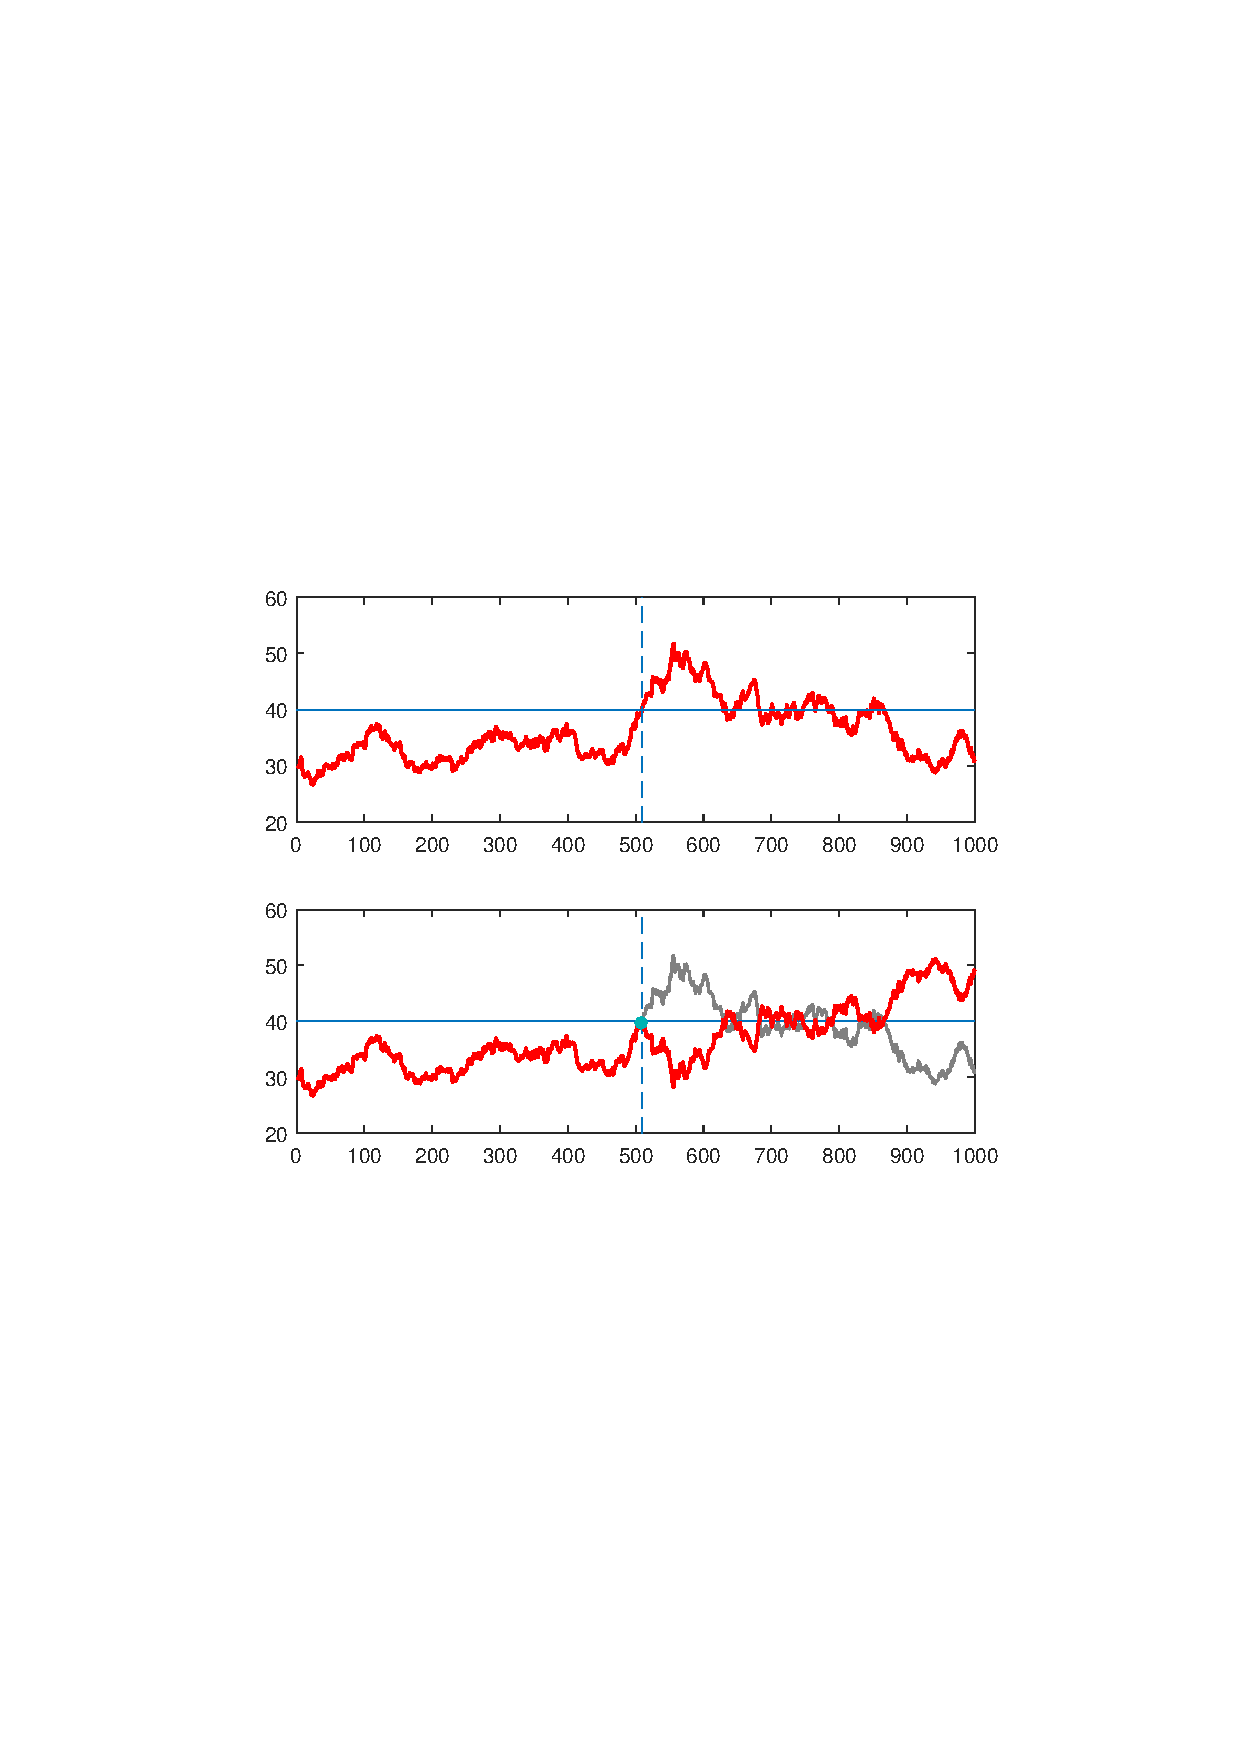
\includegraphics[scale=.7]{fig/barrier.pdf}
\end{frame}

\subsection{布朗运动的最大值}
\begin{frame}{布朗运动的最大值}
  对于布朗运动$W(t)$,若在区间$t\in[0,T]$上,有:
  $$M_T=\max_{t\in [0,T]}W(t)$$
    则称$M_T$是布朗运动在$[0,T]$上的最大值。

    当$a>0$时,如果在时间$t$处,$W(t)>a$,则意味着在时间段$[0,t]$上,$M_t>a$并且$\tau_a<t$,因此:
\begin{equation*}
\begin{split}
\{M_t>a\}&=\{M_t>a,W(t)>a\}\cup\{M_t>a, W(t)\le a\}\\
&=\{W(t)>a\}\cup\{M_t>a, W(t)\le a\}
\end{split}
\end{equation*}
由于上面的两个事件互不相容,因此:
\begin{equation*}
\Pr(M_t>a)=\Pr\qty[W(t)>a]+\Pr\qty[M_t>a, W(t)\le a]
\end{equation*}
\end{frame}


\begin{frame}{布朗运动的最大值(cont.)}
  根据反射原理,以$\tau_a$为界,当$t\ge \tau_a$时,$\widetilde{W}(t)=2a-W(t)$,于是:
  \begin{equation*}
  \Pr\qty[M_t>a, W(t)\le a]=\Pr\qty[M_t>a,\widetilde W(t)\ge a]=\Pr\qty[\widetilde W(t)\ge a]
  \end{equation*}
  由于$\widetilde W(t)$与$W(t)$均是布朗运动,因此:
  \[\Pr\qty[\widetilde W(t)\ge a]=\Pr\qty[W(t)\ge a] \]
  于是:
  \begin{equation*}
  \begin{split}
  \Pr(M_t>a)&=\Pr\qty[W(t)>a]+\Pr\qty[W(t)\ge a]=2\cdot\Pr\qty[W(t)> a]\\
  &=2\cdot \Pr\left(Z>\frac{a}{\sqrt{t}}\right)=2\cdot \int_{a/\sqrt{t}}^{\infty} \frac{1}{\sqrt{2\pi}}\exp\left(-\frac{1}{2}x^2\right)\dif x \\
  &=2\cdot \int^{-a/\sqrt{t}}_{-\infty} \frac{1}{\sqrt{2\pi}}\exp\left(-\frac{1}{2}x^2\right)\dif x=2N\left( -\frac{a}{\sqrt{t}}\right) 
  \end{split}
  \end{equation*}
\end{frame}


\begin{frame}{布朗运动的最大值(cont.)}
    从另一个角度来看,$\{M_t>a\}$这一事件必然意味着$\{\tau_a<t\}$成立,因此:
    \begin{equation*}
    \Pr(M_t>a)=\Pr(\tau_a<t)=F_{\tau_a}(t)=2N\left( -\frac{a}{\sqrt{t}}\right) ,\qquad a>0
    \end{equation*}

    \begin{block}{提示:}
      此处直接使用了首中时刻$\tau_a$的分布函数。
    \end{block}
\end{frame}



\begin{frame}{布朗运动的最大值$M_t$的分布函数}
    \[\begin{split}
      F_{M_t}(a)&=\Pr(M_t<a)=1-\Pr(M_t>a)\\
      &=1-2N\left( -\frac{a}{\sqrt{t}}\right)\\
      &=\int^{a/\sqrt{t}}_{-a/\sqrt{t}}\frac{1}{\sqrt{2\pi}}\exp\left(-\frac{1}{2}x^2\right)\dif x
      \end{split}\]
\end{frame}

\subsection{反射原理在金融中的应用}
\begin{frame}{反射原理在金融中的应用}
  回望期权(lookback option)在未来到期日,其回报数额的计算不是依据行权价和到期日标的资产的价格:看涨型回望期权的回报数额是依据行权价和期间内标的资产价格的最高值计算确定;看跌型回望期权的回报数额则是依据到期日标的资产价格与期间内标的资产价格的最低值计算确定。对回望期权进行定价,就需要使用反射原理以及布朗运动最大值的相关性质。

  障碍期权的定价问题当中,敲入或敲出的条件可以等价为判断期权有效期内,标的资产价格最大值或最小值是否达到障碍价格。因此,
也可以基于反射原理,最终推导出障碍期权的价格。
\end{frame}

\section{马氏过程}
\begin{frame}{回顾:马氏性}
  在给定当前的条件下,未来与过去是独立的,即:
  \begin{equation*}
  \Pr(X_{n+1}=j|X_n=i, X_k=x_k, 0\le k< n)=\Pr(X_{n+1}=j|X_n=i)
  \end{equation*}
  在时间和状态均连续的布朗运动中,同样具有此种性质,即:
  \begin{equation*}
  \Pr(X_{t+s}\le y|X_u, 0\le u\le s)=\Pr(X_{t+s}\le y|X_s)
  \end{equation*}
  当这个条件概率不依赖于$s$的取值时,该过程具有时齐性,即:
  \begin{equation*}
  \Pr(X_{t+s}\le y|X_s)=\Pr(X_{t}\le y|X_0),\qquad \forall s
  \end{equation*}

  \begin{block}{}
    在时间和状态均连续的过程中,若满足马氏性,则称其为马氏过程。相应地,$\Pr(X_{t}\le y|X_0=x)$称为过程的转移分布函数。
  \end{block}
\end{frame}


\begin{frame}{转移函数}
  正如离散状态马氏链当中,转移矩阵在研究随机演化的过程中扮演着重要的角色,马氏过程则是使用转移函数来研究过程随时间的演化。转移函数也称
  转移核(transition kernel),记作$K_t(x,\cdot )$,表示在$X_0=x$的条件下,经过时间$t$到达$X_t$处的条件概率密度。因此下式成立:
  \begin{equation*}
  \Pr(X_{t}\le y|X_0=x)=\int^{y}_{-\infty} K_t(x,w)\dif w
  \end{equation*}
\end{frame}


\begin{frame}{C-K方程}
  正如离散状态马氏链满足C-K方程,马氏过程同样具有类似的C-K方程,只不过原先公式中的求和符号变成了积分符号;原先的转移概率变成了转移核。
  
  离散状态马氏链中的转移概率$p_{s+t}(x,y)$与马氏过程中的转移核$K_{s+t}(x,y)$之间的关系如下:
  \begin{align*}
  p_{s+t}(x,y)&=\sum_k p_s(x,k)p_t(k,y), \qquad \forall k\\
  K_{s+t}(x,y)&=\int_{-\infty}^{\infty}K_s(x,z)K_t(z,y)\dif z, \qquad \forall s,t
  \end{align*}
\end{frame}


\begin{frame}{布朗运动的转移函数}
  对于布朗运动$W(t)$而言,由于$W(t+s)-W(s)=W(t)\sim \mathcal{N}(0,t)$,因此:
  \[\begin{split}
  \Pr\qty[W(s+t)\le y|W(s)=x]&=\Pr\qty[W(t)\le (y-x)|W(0)=0]\\
  &=\int^{y-x}_{-\infty} \frac{1}{\sqrt{2\pi t}}\exp\left(-\frac{w^2}{2t}\right)\dif w
  \end{split} \]
  从而: 
  \begin{equation*}
  K_t(x,y)=\frac{1}{\sqrt{2\pi t}}\exp\left[-\frac{(y-x)^2}{2t}\right]
  \end{equation*} 
\end{frame}


\section{布朗运动的变化形式}

\subsection{布朗桥}
\begin{frame}{布朗桥的定义1}
  假设$W(t)$是一个布朗运动,令
  \begin{equation*}
  W^*(t)=W(t)-tW(1),\qquad t\in[0,1]
  \end{equation*}
  则称$W^*(t)$为布朗桥(Brownian bridge)。

  根据定义不难看出:
\begin{equation*}
W^*(0)=W(0)=0,\qquad W^*(1)=W(1)-W(1)=0
\end{equation*}
可见,$W^*(t)$的两个端点是固定的,就如同桥一样,故名布朗桥。
\end{frame}





\begin{frame}{布朗桥$W^*(t)$的期望和协方差}
  对于布朗桥$W^*(t)$,假设$0\le s\le t\le 1$,其期望和协方差分别为:
  \begin{equation*}
  \E[W^*(t)]=\E[W(t)]-\E[tW(1)]=\E[W(t)]-t\E[W(1)]=0
  \end{equation*}
  \begin{equation*}
  \begin{split}
  \Cov[W^*(s)W^*(t)]&=\E[W^*(s)W^*(t)]=\E\left[W(s)-sW(1)\right]\left[W(t)-tW(1)\right]\\
  &=\E[W(s)W(t)]-t\E[W(s)W(1)]\\
  &\quad -s\E[W(1)W(t)]+ts\E[W^2(1)]\\
  &=s-ts-st+ts=s-ts=s(1-t)
  \end{split}
  \end{equation*}
\end{frame}


\begin{frame}{布朗桥的定义2}
  假设$W(t)$是一个布朗运动,令
  \begin{equation*}
  X(t)=W(t)-\frac{t}{T}W(T),\qquad t\in[0,T]
  \end{equation*}
  则称$X(t)$为布朗桥。

  此处定义的布朗桥仍然满足$X(0)=X(T)=0$,可以看作定义1的拓展。不难看出,当$T=1$时,布朗桥$X(t)$就变成了$W^*(t)$。
\end{frame}


\begin{frame}{布朗桥$X(t)$的期望和协方差}
  假设$0\le s\le t\le T$
  ,可以得到$X(t)$的期望和协方差分别为:
  \begin{equation*}
  \E[X(t)]=\E[W(t)]-\frac{t}{T}\E[W(T)]=0
  \end{equation*}
  \begin{equation*}
  \begin{split}
  \Cov[X(s)X(t)]&=\E[X(s)X(t)]=\E\left[W(s)-\frac{s}{T}W(T)\right]\left[W(t)-\frac{t}{T}W(T)\right]\\
  &=\E[W(s)W(t)]-\frac{t}{T}\E[W(s)W(T)]\\
  &\quad -\frac{s}{T}\E[W(T)W(t)]+\frac{st}{T^2}\E[W^2(T)]\\
  &=s-\frac{t}{T}s-\frac{s}{T}t+\frac{st}{T^2}T\\
  &=s-\frac{st}{T}
  \end{split}
  \end{equation*}
\end{frame}


\begin{frame}{布朗桥的定义3}
  假设$W(t)$是一个布朗运动。给定$T>0$,$a,b\in\mathbb{R}$,则在$[0,T]$上从$a$到$b$的布朗桥$X^{a\to b}(t)$定义如下:
  \begin{equation*}
  X^{a\to b}(t)=a+(b-a)\cdot \frac{t}{T}+X(t), \qquad t\in[0,T]
  \end{equation*}
  其中,$X(t)$是由$X(t)=W(t)-\frac{t}{T}W(T)$定义的布朗桥,满足$X(0)=X(T)=0$。

  布朗桥$X^{a\to b}(t)$的两个端点$0$与$T$满足下式:
\[X^{a\to b}(0)=a,\qquad X^{a\to b}(T)=b \]
\end{frame}


\begin{frame}{$X^{a\to b}(t)$的期望和协方差}
  \begin{equation*}
    \E[X^{a\to b}(t)]=a+(b-a)\cdot \frac{t}{T}+\E[X(t)]=a+(b-a)\cdot \frac{t}{T}
    \end{equation*}
    由于$X^{a\to b}(t)$的表达式中,$a+(b-a)\cdot \dfrac{t}{T}$是确定项(deterministic term),因此计算协方差时可以不予考虑。于是$X^{a\to b}(t)$的协方差就与$X(t)$的相同,即:
    \begin{equation*}
    \Cov[X^{a\to b}(s)X^{a\to b}(t)]=\Cov[X(s)X(t)]=s-\frac{st}{T}
    \end{equation*}
\end{frame}


\begin{frame}{布朗桥的图示}
  \centering
	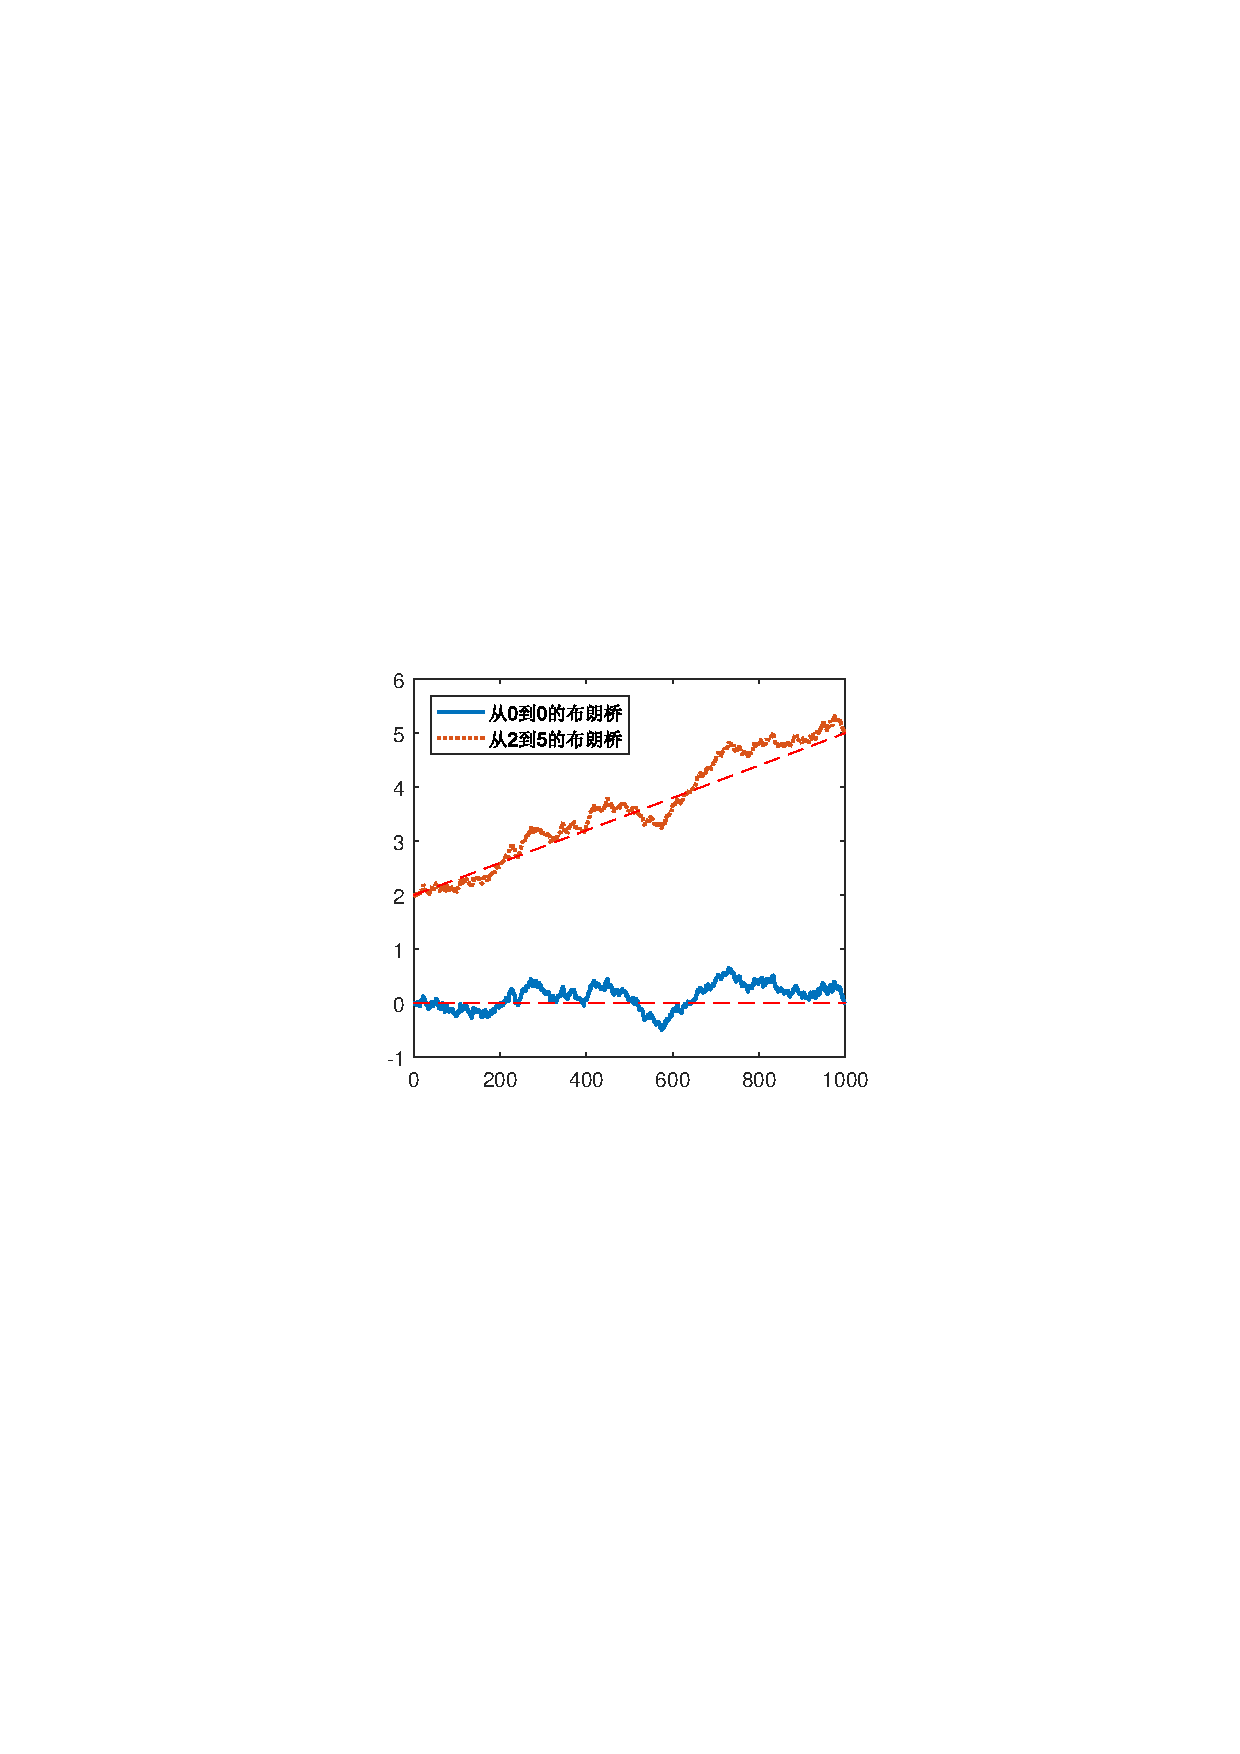
\includegraphics[scale=1]{fig/bb1.pdf}
\end{frame}

\subsection{有漂移的布朗运动}
\begin{frame}{有漂移的布朗运动}
  假设$W(t)$是一个布朗运动,则以下随机过程$X(t)$称为有漂移的布朗运动(Brownian motion with drift):
  \begin{equation*}
  X(t)=\mu t+\sigma W(t), \qquad t\ge 0
  \end{equation*}
  其中的常数$\mu$称为漂移系数(drift),常数$\sigma$称为波动率(volatility)。

  对$X(t)$计算期望和方差,结果如下:
\begin{equation*}
\begin{split}
\E[X(t)]&=\E(\mu t)+\E[\sigma W(t)]=\mu t\\
\Var[X(t)]&=\Var[\mu t+\sigma W(t)]=\Var[\sigma W(t)]=\sigma^2 t
\end{split}
\end{equation*}
\end{frame}



\begin{frame}{不同形式的布朗运动对比}
  \centering 
	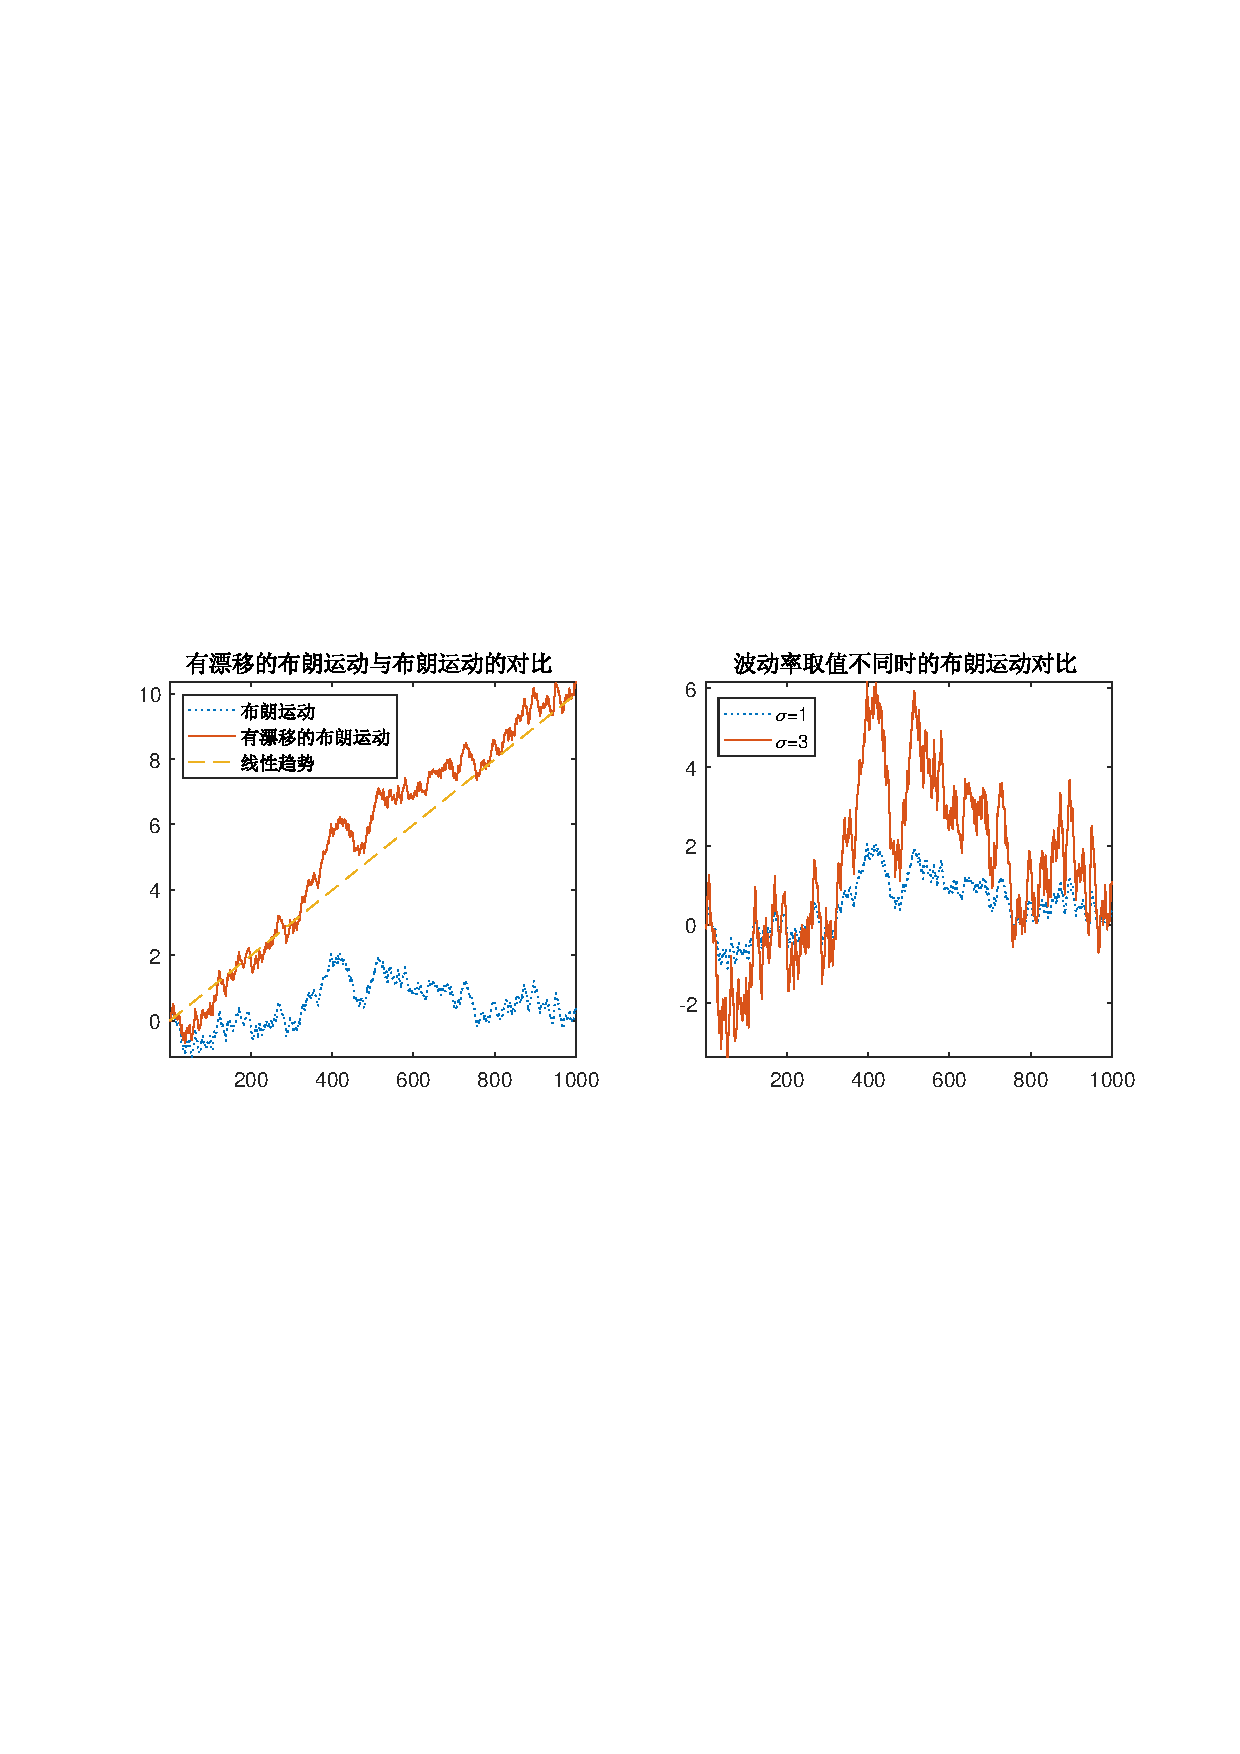
\includegraphics[height=.65\textheight]{fig/drift.pdf}
\end{frame}

\subsection{几何布朗运动}
\begin{frame}{几何布朗运动}
  几何布朗运动的状态空间是$\mathbb{R}^+\cup\{0\}$,即它是一个非负的过程。几何布朗运动在数理金融中应用非常广泛,可以用来对股票等金融资产进行建模。
\normalsize
  \begin{block}{定义:}
    假设$X(t)$是漂移系数为$\mu$、波动率为$\sigma$的布朗运动,即:
    \[X(t)=\mu t+\sigma W(t) \]
    定义过程$G(t)$,其满足:
    \begin{equation*}
    G(t)=G(0)\exp[X(t)],\qquad t\ge 0
    \end{equation*}
    并且$G(0)>0$,则称$G(t)$是几何布朗运动(geometric Brownian motion)。 
  \end{block}
\end{frame}



\end{document}